%%%%%%%%%%%%%%%%%%%%%%%%%%%%%%%%%%%%%%%%%%%%%%%%%%
\begin{frame}{Überblick über die Präsentation}

\begin{itemize}
\onslide<1,4>

	\item Motivation
	\begin{itemize}
		\item Wen geht es an?
		\item Welche Probleme werden adressiert?
	\end{itemize}

\onslide<2,4>

	\item Ziel
	\begin{itemize}
		\item Was erhalten wir, wenn wir das richtig anwenden?
	\end{itemize}

\onslide<3,4>

	\item Weg
	\begin{itemize}
		\item Wie kommen wir dahin?
	\end{itemize}
\end{itemize}

\end{frame}


%%%%%%%%%%%%%%%%%%%%%%%%%%%%%%%%%%%%%%%%%%%%%%%%%%
\begin{frame}{Software aus verschiedenen Perspektiven}

\begin{itemize}

\onslide<1,4>
	
	\item Auftraggeber:

	\begin{itemize}
		\item \glqq Die Software soll tun, was ich erwarte.\grqq
		\item \glqq Ich will das Ganze möglichst preiswert.\grqq
	\end{itemize}
	
\onslide<2,4>
	
	\item Entwickler:
	
	\begin{itemize}
		\item \glqq Ich will wissen, was ich entwickeln soll.\grqq
		\item \glqq Wann bin ich fertig?\grqq
	\end{itemize}
	
\onslide<3,4>
	
	\item Nach der Lieferung:
	
	\begin{itemize}
		\item \glqq Was macht die Software genau?\grqq
		\item \glqq Bug oder Feature?\grqq
	\end{itemize}
\end{itemize}

\end{frame}


%%%%%%%%%%%%%%%%%%%%%%%%%%%%%%%%%%%%%%%%%%%%%%%%%%
\begin{frame}{Die Vision -- Eine Quelle für alle}

\begin{itemize}
	\item Beschreibung der Anforderung
	\begin{itemize}
		\item Alle sollen das gleiche Verständnis haben.
	\end{itemize}

\onslide+<2->
	
	\item Akzeptanztests für die Entwicklung
	\begin{itemize}
		\item Überprüfbare Kriterien
		\item Werden im Laufe der Entwicklung \glqq begrünt\grqq
	\end{itemize}

\onslide+<3->
	
	\item Ausführbare Dokumentation
	\begin{itemize}
		\item Sicherstellen, dass die Dokumentation zur Anwendung passt.
		\item Hilfestellung bei Supportfällen
	\end{itemize}
\end{itemize}

\onslide+<4->
Wir brauchen:	
$\Rightarrow$ Single Source of Truth

\end{frame}


%%%%%%%%%%%%%%%%%%%%%%%%%%%%%%%%%%%%%%%%%%%%%%%%%%
\begin{frame}{Was wir dazu brauchen}

\begin{itemize}
	\item Ein einziges Repository für die Informationen
	\item Mit Beschreibung \em und \em Tests
	\item In einer für jeden verständlichen Formulierung
	\item Integriert mit der Anwendung, damit durch die Tests die Konsistenz mit der Anwendung verifiziert werden kann.
\end{itemize}

\end{frame}

%%%%%%%%%%%%%%%%%%%%%%%%%%%%%%%%%%%%%%%%%%%%%%%%%%
\begin{frame}{Wie wir dahin kommen}

\begin{itemize}
	\item Kommunikation und Zusammenarbeit \em aller \em Beteiligten 
	\begin{itemize}
		\item Es entsteht ein gemeinsames Verständnis
		\item Stille Annahmen werden explizit
		\item Es fliessen unterschiedliche Sichtweisen und Erfahrungen ein
	\end{itemize}
	
	\item Fokus
	\begin{itemize}
		\item Konzentration auf die fachlich wichtigen Aspekte
		\item Das Ziel muss sein, die Single Source of Truth zu schaffen
	\end{itemize}
\end{itemize}

\onslide+<2->
	
$\Rightarrow$ Specification Workshops

\end{frame}


%%%%%%%%%%%%%%%%%%%%%%%%%%%%%%%%%%%%%%%%%%%%%%%%%%
\begin{frame}{Ein Workshop ist notwendig, weil}

\begin{itemize}
	\item Direkte Kommunikation und Diskussion der Teilnehmer fördern
	\begin{itemize}
		\item Schnellen Informationsfluss durch Fragen und direkte Antworten
		\item Entdecken von Widersprüchen, Lücken, Mißverständnissen
		\item Gemeinsames Verständnis
	\end{itemize}

	\item Die zeitliche Begrenzung betont
	\begin{itemize}
		\item Die Wichtigkeit, zu einem Ergebnis zu kommen
		\item Den Fokus
		\item Ein strukturiertes Vorgehen
	\end{itemize}
\end{itemize}

\end{frame}


%%%%%%%%%%%%%%%%%%%%%%%%%%%%%%%%%%%%%%%%%%%%%%%%%%
\begin{frame}{Specification Workshop}

\begin{itemize}
	\item Teilnehmer: 
	\begin{itemize}
		\item Auftraggeber, Kunde, Product Owner
		\item Entwickler
		\item Tester, QA-Personen
	\end{itemize}
	\item Zeit: 
	\begin{itemize}
		\item Unbedingtes Timeboxing
		\item ca. 4 Stunden für 2 Wochen Entwicklung
	\end{itemize}
	\item Durchführung mit Moderator: 
	\begin{itemize}
		\item Fokussierung
		\item Ergebniserreichung
	\end{itemize}
\end{itemize}

\end{frame}



%%%%%%%%%%%%%%%%%%%%%%%%%%%%%%%%%%%%%%%%%%%%%%%%%%
\begin{frame}{So kann ein Specification Workshop ablaufen}

\begin{enumerate}
	\item Der Auftraggeber beschreibt sein zu lösendes Problem
	\item Die Teilnehmer befragen ihn, um Klarheit zu erhalten
	\item Die Teilnehmer erarbeiten Beispiele
	\item Die Beispiele werden zusammengeführt und auf das Wesentliche reduziert
	\item Aus den Beispielen wird eine Spezifikation abgeleitet
\end{enumerate}

\end{frame}


%%%%%%%%%%%%%%%%%%%%%%%%%%%%%%%%%%%%%%%%%%%%%%%%%%
\begin{frame}{Was ein Specification Workshop \em nicht \em ist}

\begin{itemize}
	\item Der Workshop ist kein Meeting
	\begin{itemize}
		\item Es geht darum, Ergebnisse zu erzielen
	\end{itemize}
	
	\item Der Workshop ist keine Präsentation
	\begin{itemize}
		\item Die Teilnehmer sollen miteinander das Ergebnis erarbeiten
	\end{itemize}
	
	\item Der Workshop ist keine Design Session
	\begin{itemize}
		\item Es geht darum, fachliche Klarheit zu erzielen. Design ist Sache der Entwickler
	\end{itemize}
	
\end{itemize}

\onslide+<2->
	
$\Rightarrow$ Es ist Aufgabe des Moderators, dies sicherzustellen

\end{frame}


%%%%%%%%%%%%%%%%%%%%%%%%%%%%%%%%%%%%%%%%%%%%%%%%%%
\begin{frame}{Darauf sollte man achten}

\begin{itemize}
	\item Komplizierte Beispiele
	\begin{itemize}
		\item Wo liegt die Ursache der Kompliziertheit?
		\item Es geht vermutlich einfacher
		\item Oft hilft ein Aufteilen nach Aspekten
	\end{itemize}
	
\onslide+<2->
	
	\item Namensgebung
	\begin{itemize}
		\item Alle wesentlichen Konzepte brauchen klare fachlich verständliche Namen
		\item Jeder soll unter einem Begriff dasselbe verstehen
		\item Ein verwendeter Begriff muss in der gesamten Anwendung dieselbe Bedeutung haben
	\end{itemize}
	
\onslide+<3->
	
	\item Formeln
	\begin{itemize}
		\item Oft verschleiern Formeln wichtige Details
		\item Formeln müssen hinterfragt und verstanden werden
	\end{itemize}
	
\onslide+<4->
	
	\item Bei vielen Teilnehmern sollte man die Erstellung der Beispiele in Kleingruppen delegieren
\end{itemize}

\end{frame}



%%%%%%%%%%%%%%%%%%%%%%%%%%%%%%%%%%%%%%%%%%%%%%%%%%
\begin{frame}{Wie man Beispiele in Akzeptanztests umsetzen kann}

\begin{itemize}
	\item Im Idealfall sollten die Beispiele direkt als Tests ausführbar sein
	\item Sie müssen für alle Beteiligten lesbar sein
	\item Sie sollten sich auf das Notwendige beschränken. Kein Gluecode.
	\item Es existieren Frameworks, um in möglichst \glqq untechnischer\grqq Form Tests zu schreiben:
	\begin{itemize}
		\item BDD-Tools wie Cucumber (http://cukes.info)
		\item Webbasiert wie Concordion (http://www.concordion.org)
		\item Tabellenbasiert wie Fitnesse (http://www.fitnesse.org)
	\end{itemize}
\end{itemize}

\end{frame}


%%%%%%%%%%%%%%%%%%%%%%%%%%%%%%%%%%%%%%%%%%%%%%%%%%
\begin{frame}{Cucumber}
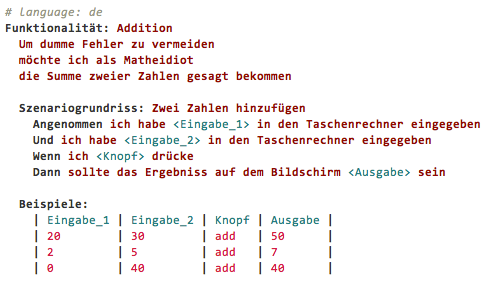
\includegraphics[width=\textwidth]{Cucumber.png} \newline
\end{frame}


%%%%%%%%%%%%%%%%%%%%%%%%%%%%%%%%%%%%%%%%%%%%%%%%%%
\begin{frame}{Concordion}
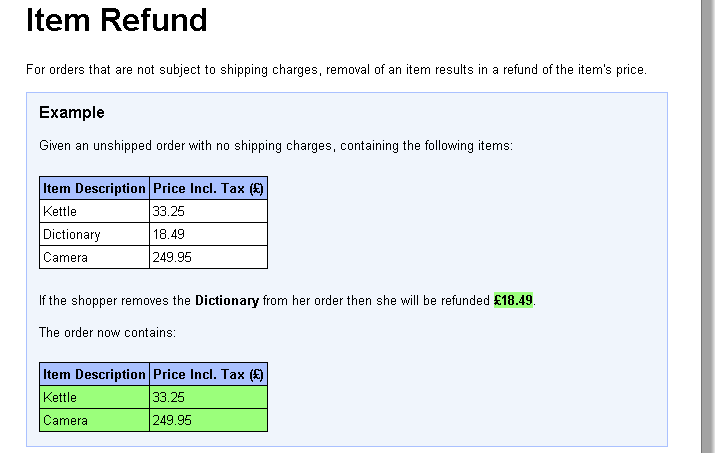
\includegraphics[width=\textwidth]{Concordion.png} \newline
\end{frame}


%%%%%%%%%%%%%%%%%%%%%%%%%%%%%%%%%%%%%%%%%%%%%%%%%%
\begin{frame}{Fitnesse}
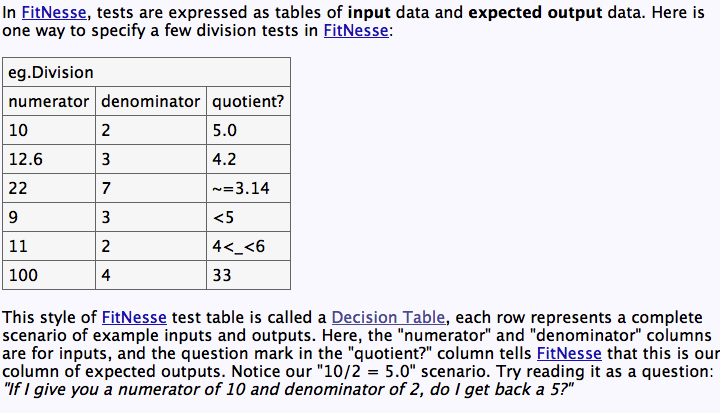
\includegraphics[width=\textwidth]{Fitnesse.png} \newline
\end{frame}



%%%%%%%%%%%%%%%%%%%%%%%%%%%%%%%%%%%%%%%%%%%%%%%%%%
\begin{frame}{Von den Beispielen hin zur Spezifikation}

\begin{itemize}
	\item Aus den Beispielen wird die Spezifikation abgeleitet und gegen die Eingangsfragen geprüft
	\item Dadurch kann man die Vollständigkeit in beide Richtungen prüfen
	\item Die Spezifikation ist genau dann gut, wenn sie auch jemand versteht, der nicht am Workshop teilgenommen hat
	\item Die Beschreibung soll eine Zusammenfassung der Beispiele sein
	\item Der Titel sollte heissen wie die Eingabe einer Suchanfrage
	\item Index und Glossar müssen aktualisiert werden
\end{itemize}

\end{frame}
 
%%%%%%%%%%%%%%%%%%%%%%%%%%%%%%%%%%%%%%%%%%%%%%%%%%
\begin{frame}{Beispiel: Konkrete Anforderung}

\begin{itemize}
	\item Ich bin Inhaber eines Hot Dog Standes und habe schon ein kleines Kassensystem mit Bestandsverwaltung
	\item Ich möchte, dass das System automatisch Nachschub bestellt, wenn mir die Würstchen ausgehen
	
	\item Was ich schon weiss:
	\begin{itemize}
		\item Mein Lieferant braucht maximal 30 Minuten
		\item Dienstags verkaufe ich mehr Würstchen
		\item Nach 16:00 Uhr verkaufe ich nicht mehr viel
	\end{itemize}
	
	\item So bestelle ich aktuell:
	\begin{itemize}
		\item Wenn ich weniger als 10 Würstchen habe (Dienstags bei 20)
		\item Nur vor 16:00 Uhr
	\end{itemize}
\end{itemize}

\onslide+<2->
	
$\Rightarrow$ Bitte erstellt in kleinen Gruppen Beispiele!

\end{frame}

%%%%%%%%%%%%%%%%%%%%%%%%%%%%%%%%%%%%%%%%%%%%%%%%%%
\begin{frame}{Vorstellung möglicher Resultate in Fitnesse}

\begin{itemize}
	\item Ein Beispiel mit Verbesserungspotenzial
	\item Ein Beispiel mit starker Aspekttrennung
\end{itemize}

\end{frame}

%%%%%%%%%%%%%%%%%%%%%%%%%%%%%%%%%%%%%%%%%%%%%%%%%%
\begin{frame}{Schlechtes Beispiel}

\begin{center}
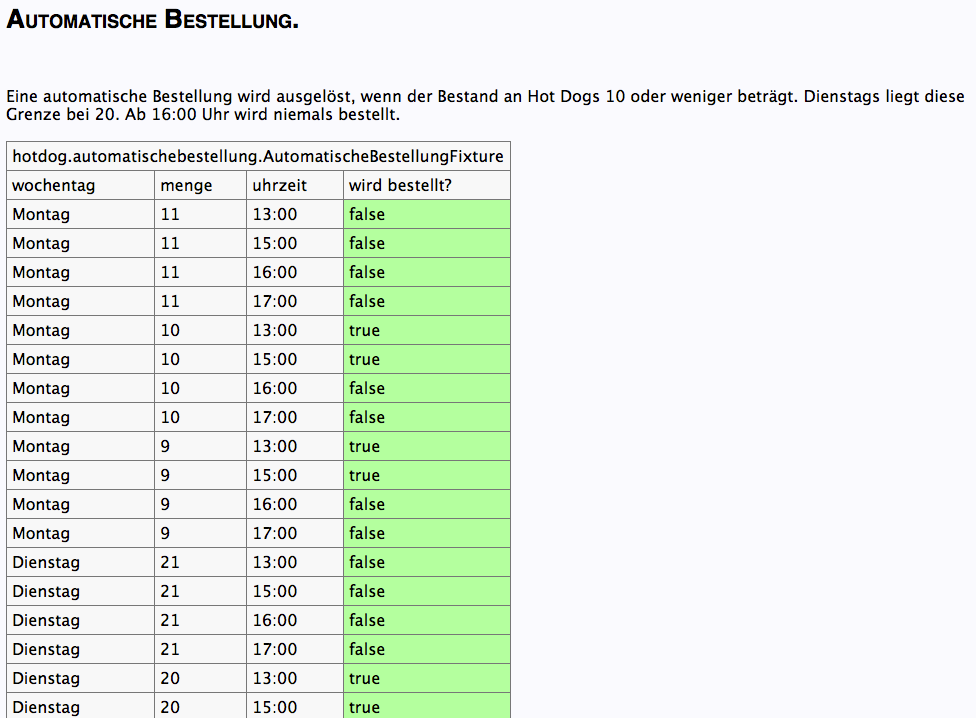
\includegraphics[height=7cm]{SchlechtesBeispiel.png} \newline
\end{center}

\end{frame}

%%%%%%%%%%%%%%%%%%%%%%%%%%%%%%%%%%%%%%%%%%%%%%%%%%
\begin{frame}{Gutes Beispiel}

\begin{center}
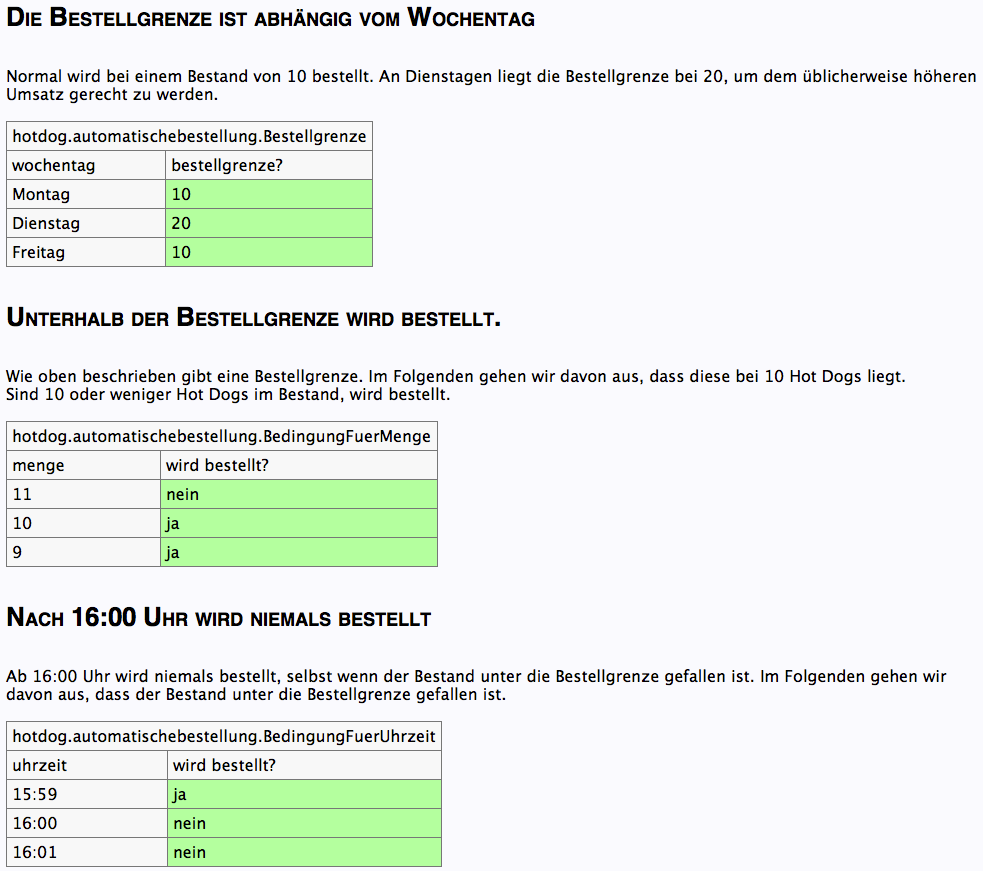
\includegraphics[height=7cm]{GutesBeispiel.png} \newline
\end{center}

\end{frame}

%%%%%%%%%%%%%%%%%%%%%%%%%%%%%%%%%%%%%%%%%%%%%%%%%%
{
\usebackgroundtemplate{
\includegraphics[width=\paperwidth,height=\paperheight]{background-slide.png}}
\begin{frame}{Vielen Dank!}

        Folien auf GitHub:
        \begin{center}
                \url{https://github.com/leider/Beispielhaft}
        \end{center}

        \begin{block}{Andreas Leidig}
        \begin{description}[Twitterxx]
                \item[E-Mail]  \href{mailto:andreas.leidig@msg-gillardon.de}{\texttt{andreas.leidig@msg-gillardon.de}}
                \item[Twitter] \href{http://twitter.com/leiderleider}{\texttt{@leiderleider}}
        \end{description}
        \end{block}

        \begin{block}{Nicole Rauch}
        \begin{description}[Twitterxx]
                \item[E-Mail]  \href{mailto:nicole.rauch@msg-gillardon.de}{\texttt{nicole.rauch@msg-gillardon.de}}
                \item[Twitter] \href{http://twitter.com/NicoleRauch}{\texttt{@NicoleRauch}}
        \end{description}
        \end{block}
\end{frame}
}
